% !TeX spellcheck = en_GB
%%%%%%%%% image SWC retrieved and MEPS %%%%%%%%%%%%%%
% !TeX spellcheck = en_GB
%\begin{landscape}
\begin{figure}[h]
	\centering
    	% 21/12
		\begin{subfigure}[b]{0.8\textwidth}
			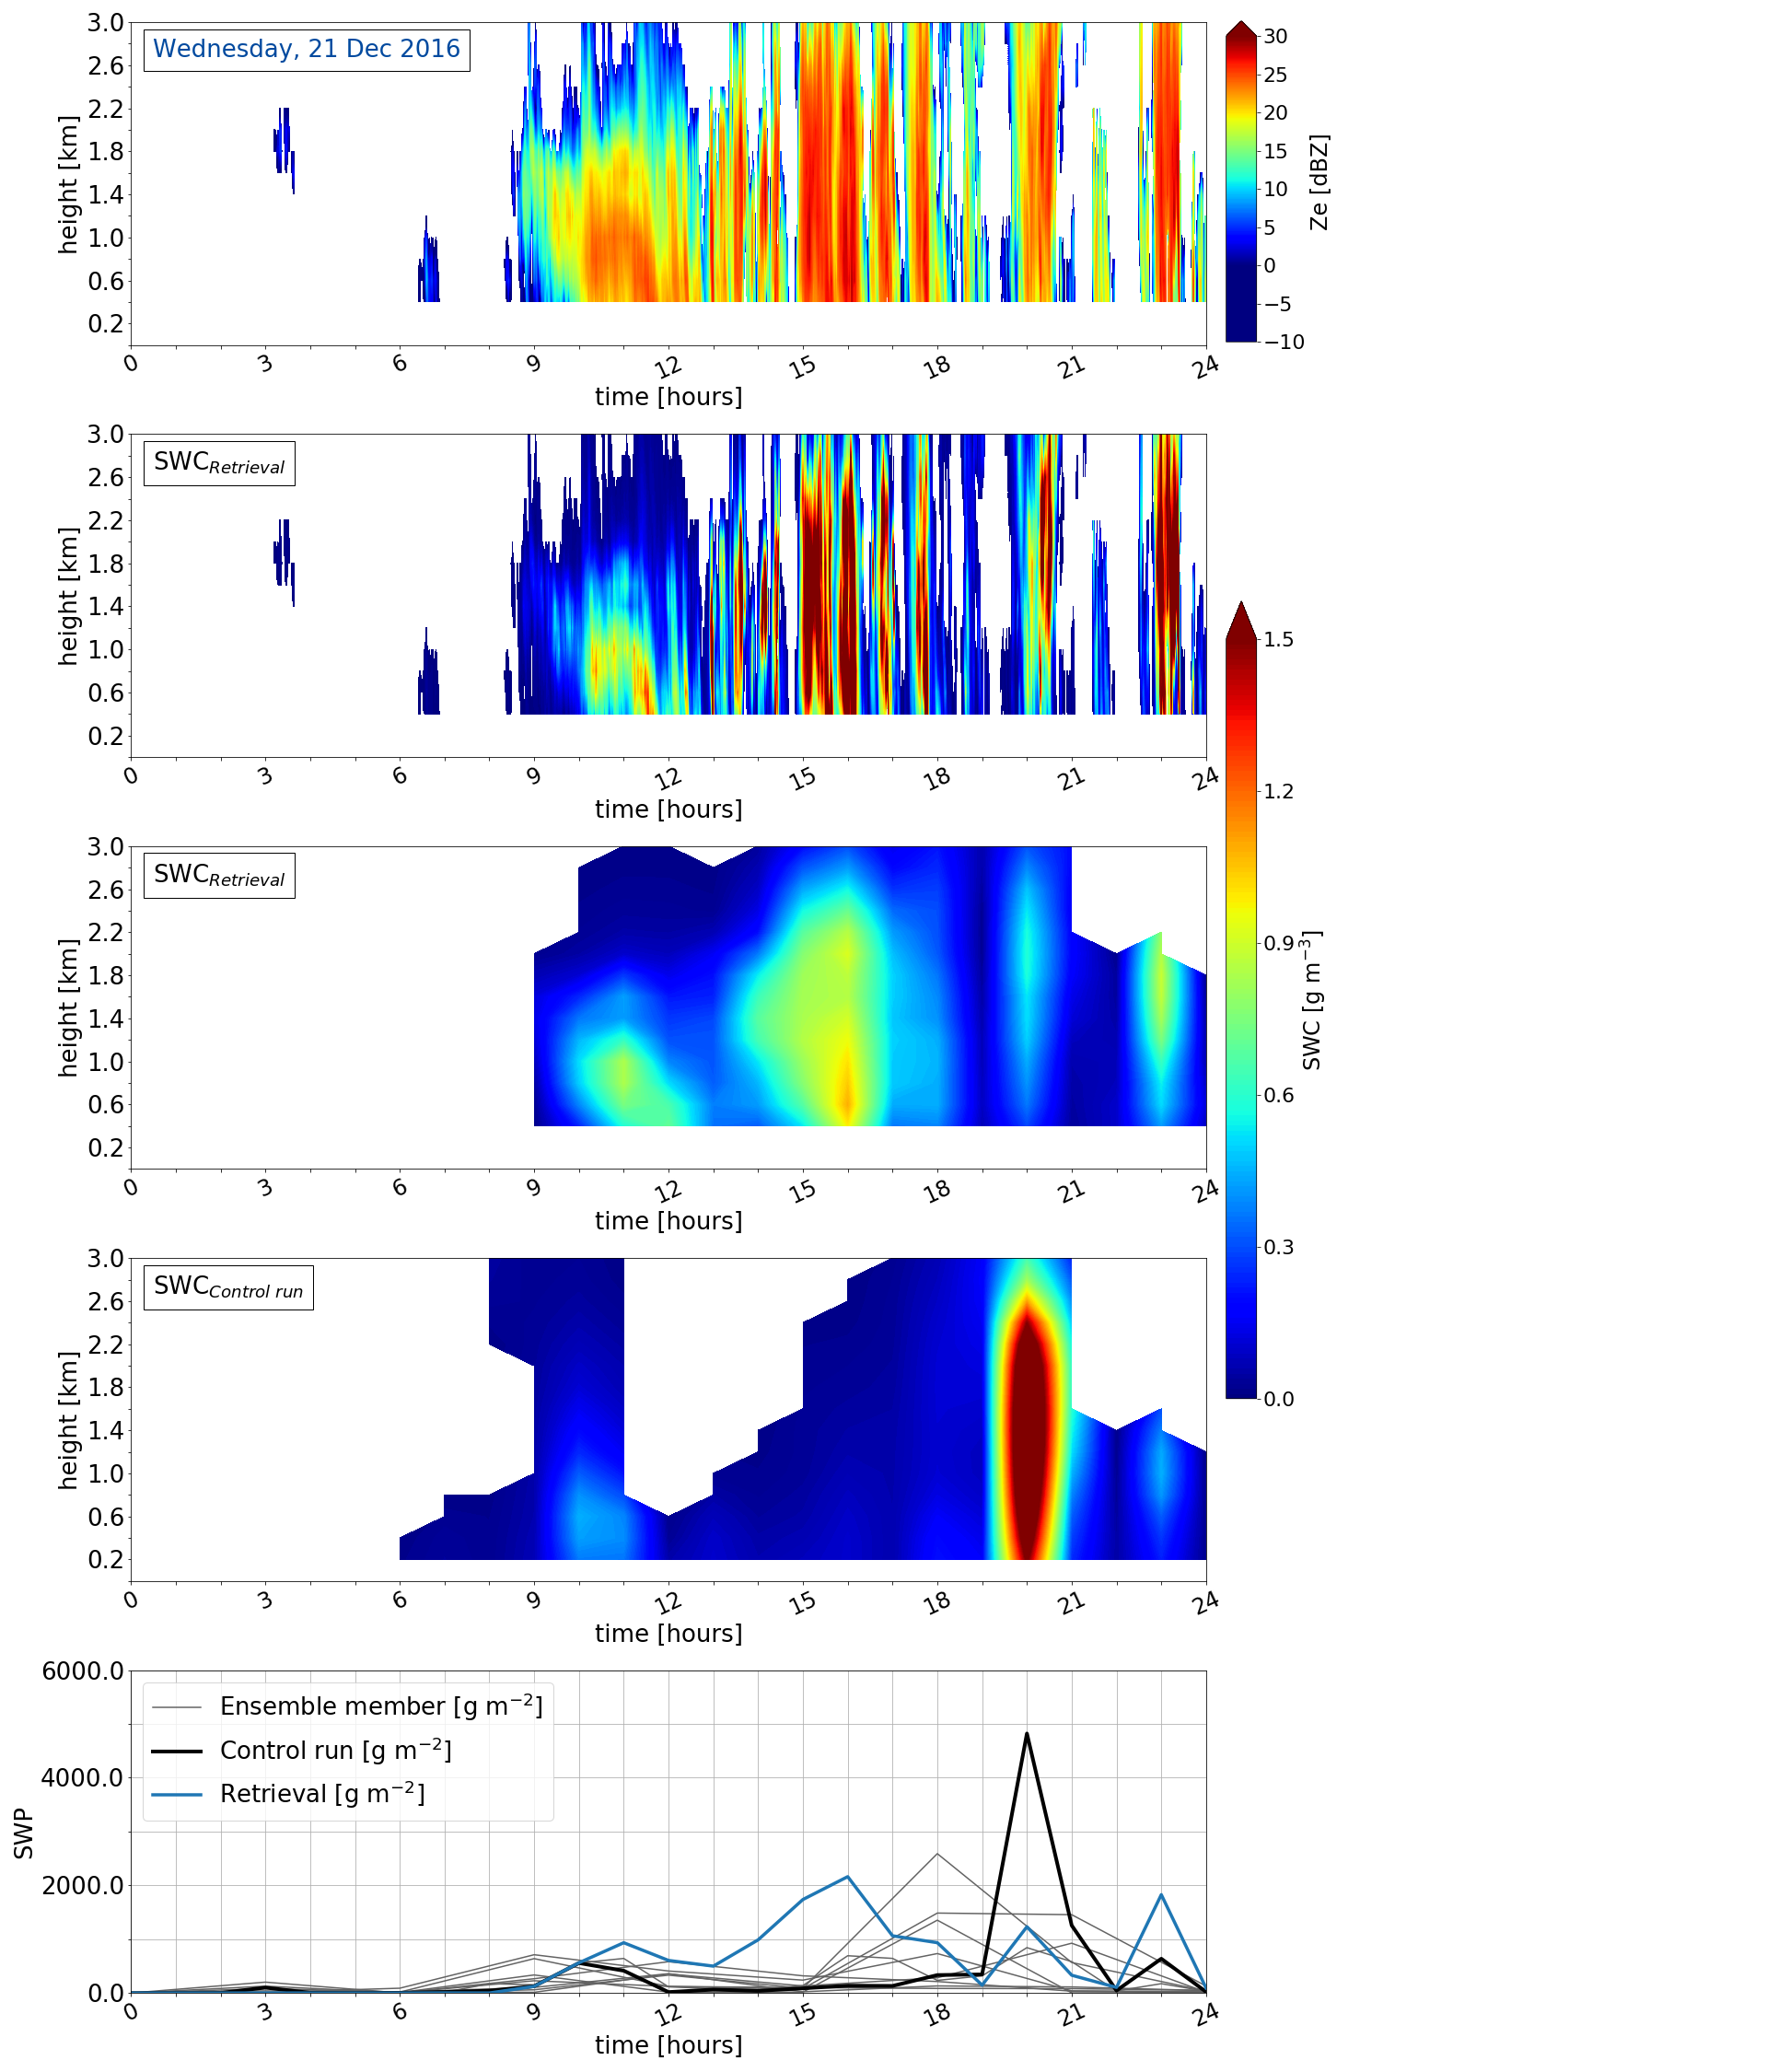
\includegraphics[trim={0.5cm 0.5cm 17.5cm .5cm},clip,width=\textwidth]{./fig_SWC/20161221}
			\caption{Wednesday, \SI{21}{\dec}}\label{fig:SWC21}
		\end{subfigure}
\end{figure}
\begin{figure}\ContinuedFloat
   	\centering
		% 22/12
	\begin{subfigure}[b]{0.8\textwidth}
			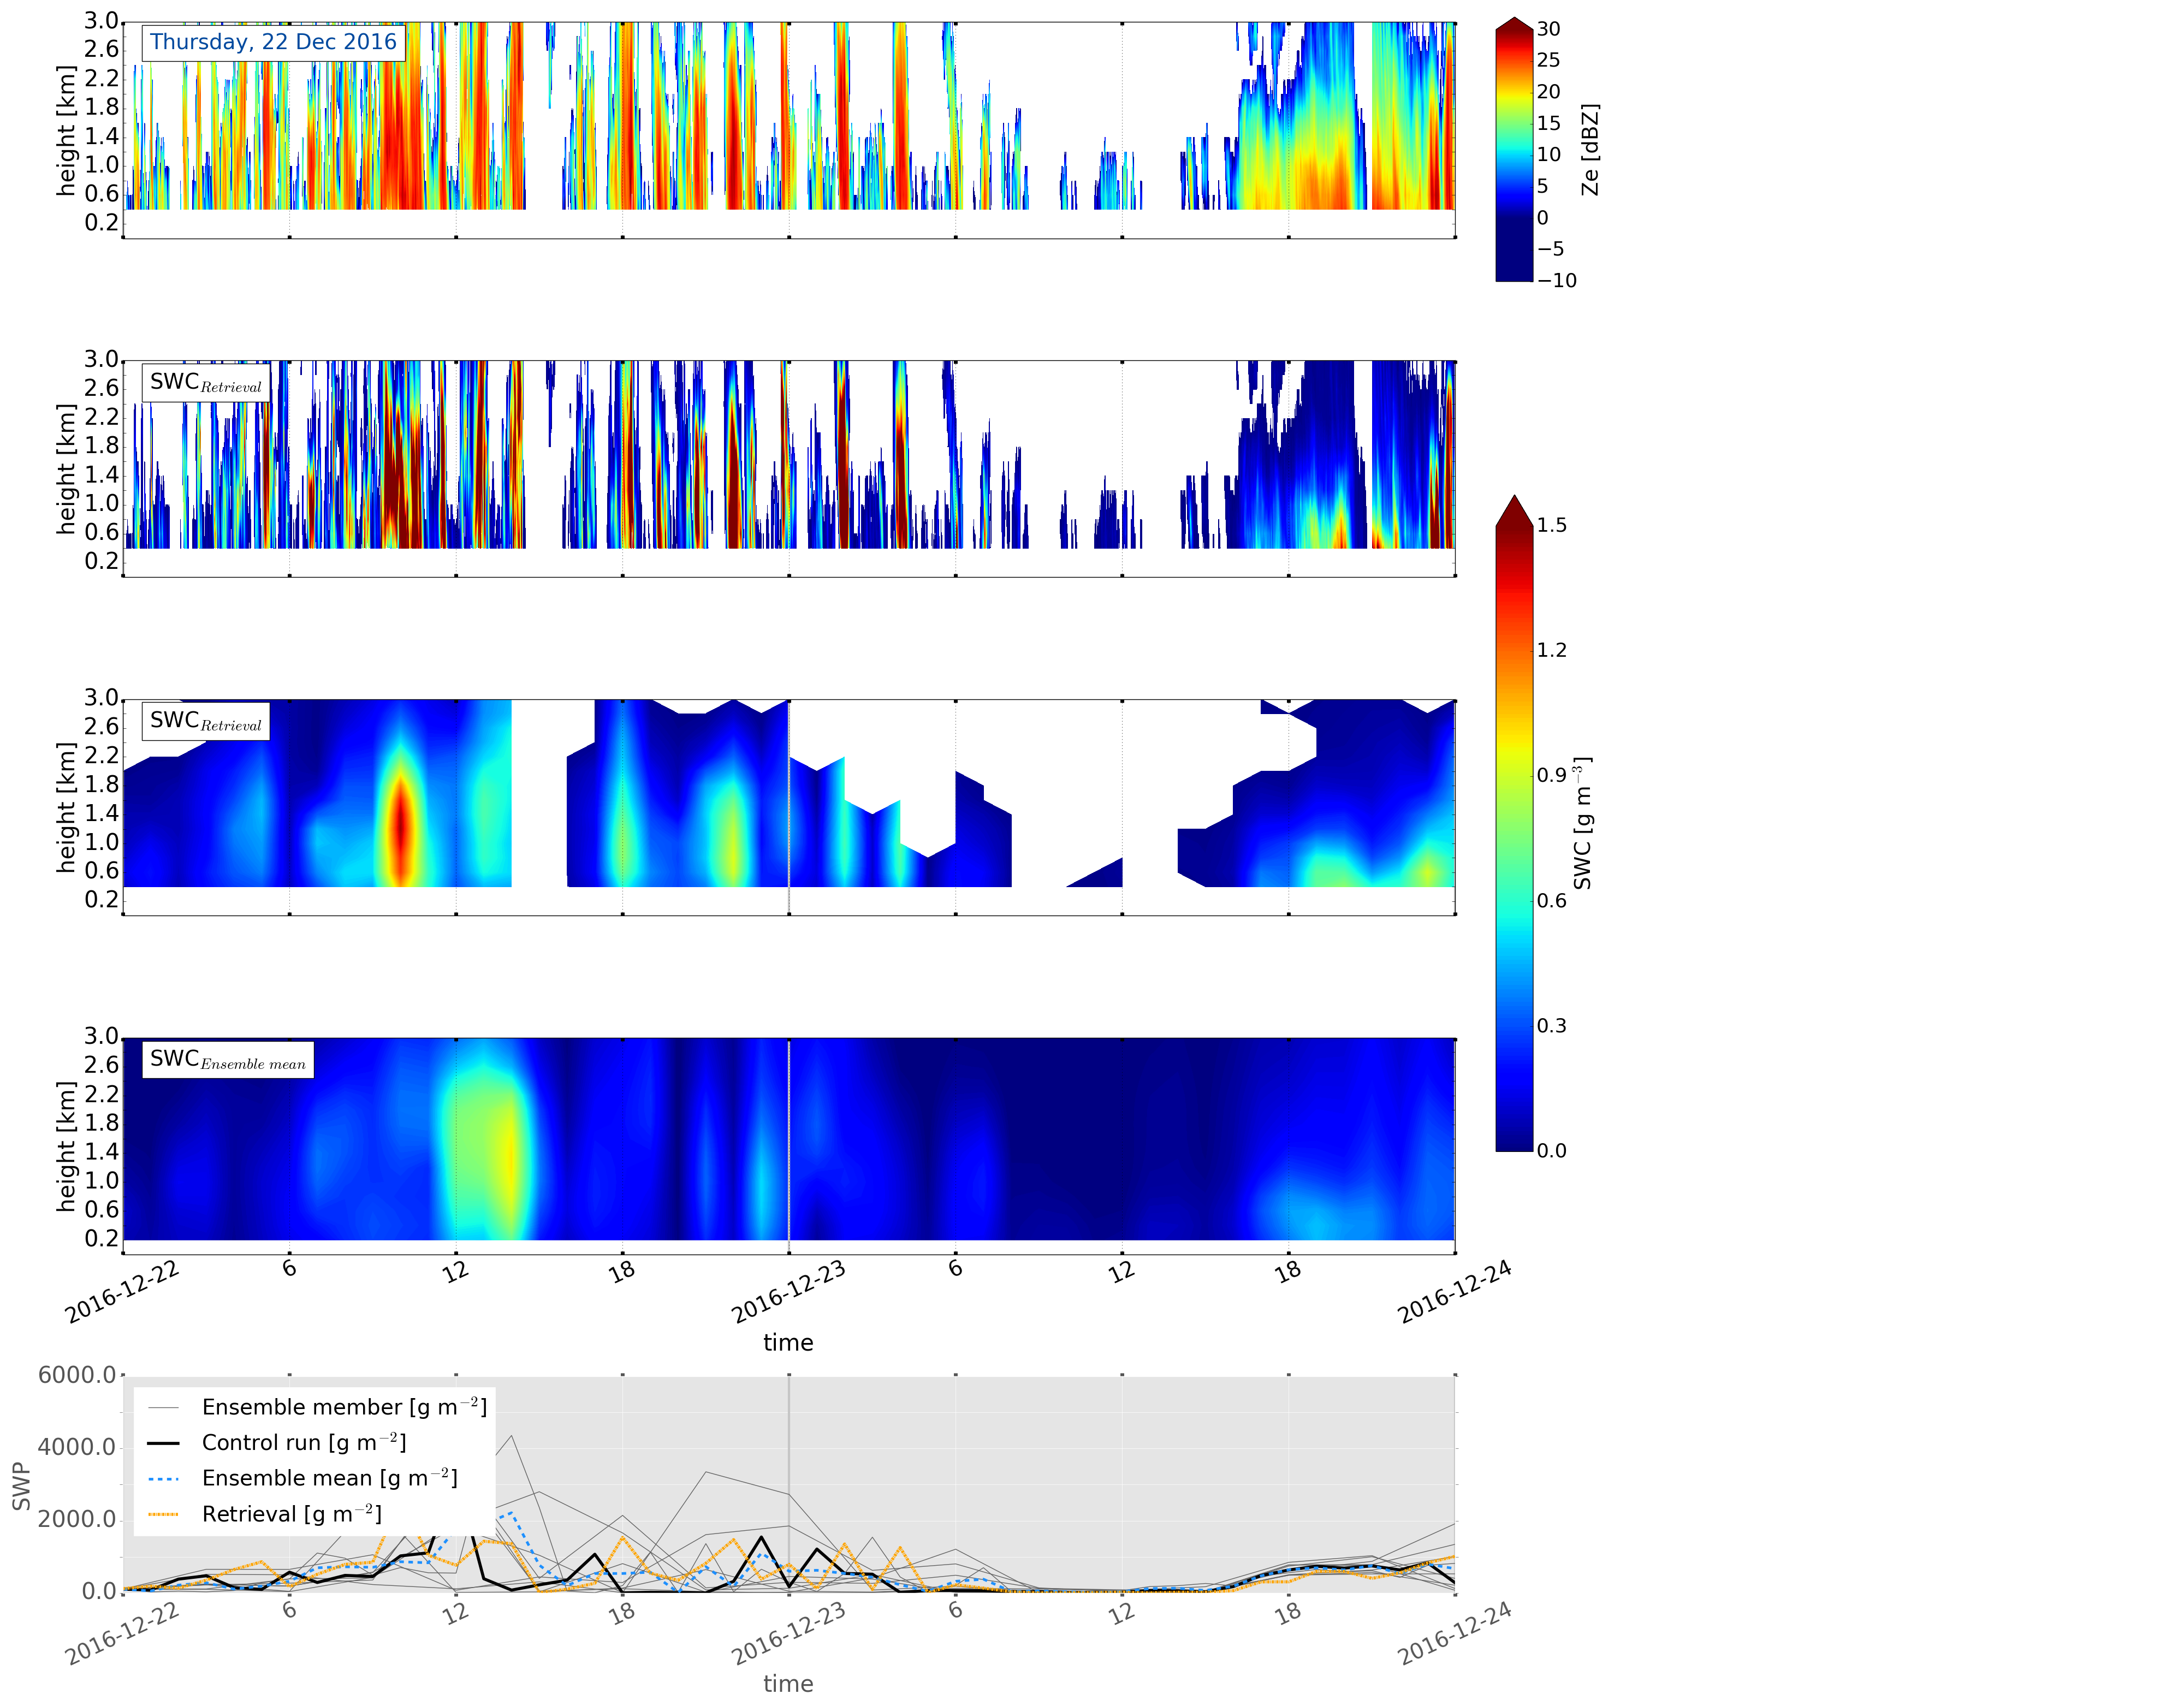
\includegraphics[trim={0.5cm 0.5cm 17.5cm .5cm},clip,width=\textwidth]{./fig_SWC/20161222}
			\caption{Thursday, \SI{22}{\dec}}\label{fig:SWC22}
		\end{subfigure}
	\end{figure}
    \begin{figure}\ContinuedFloat
   		\centering
		% 23/12
		\begin{subfigure}[b]{0.8\textwidth}
			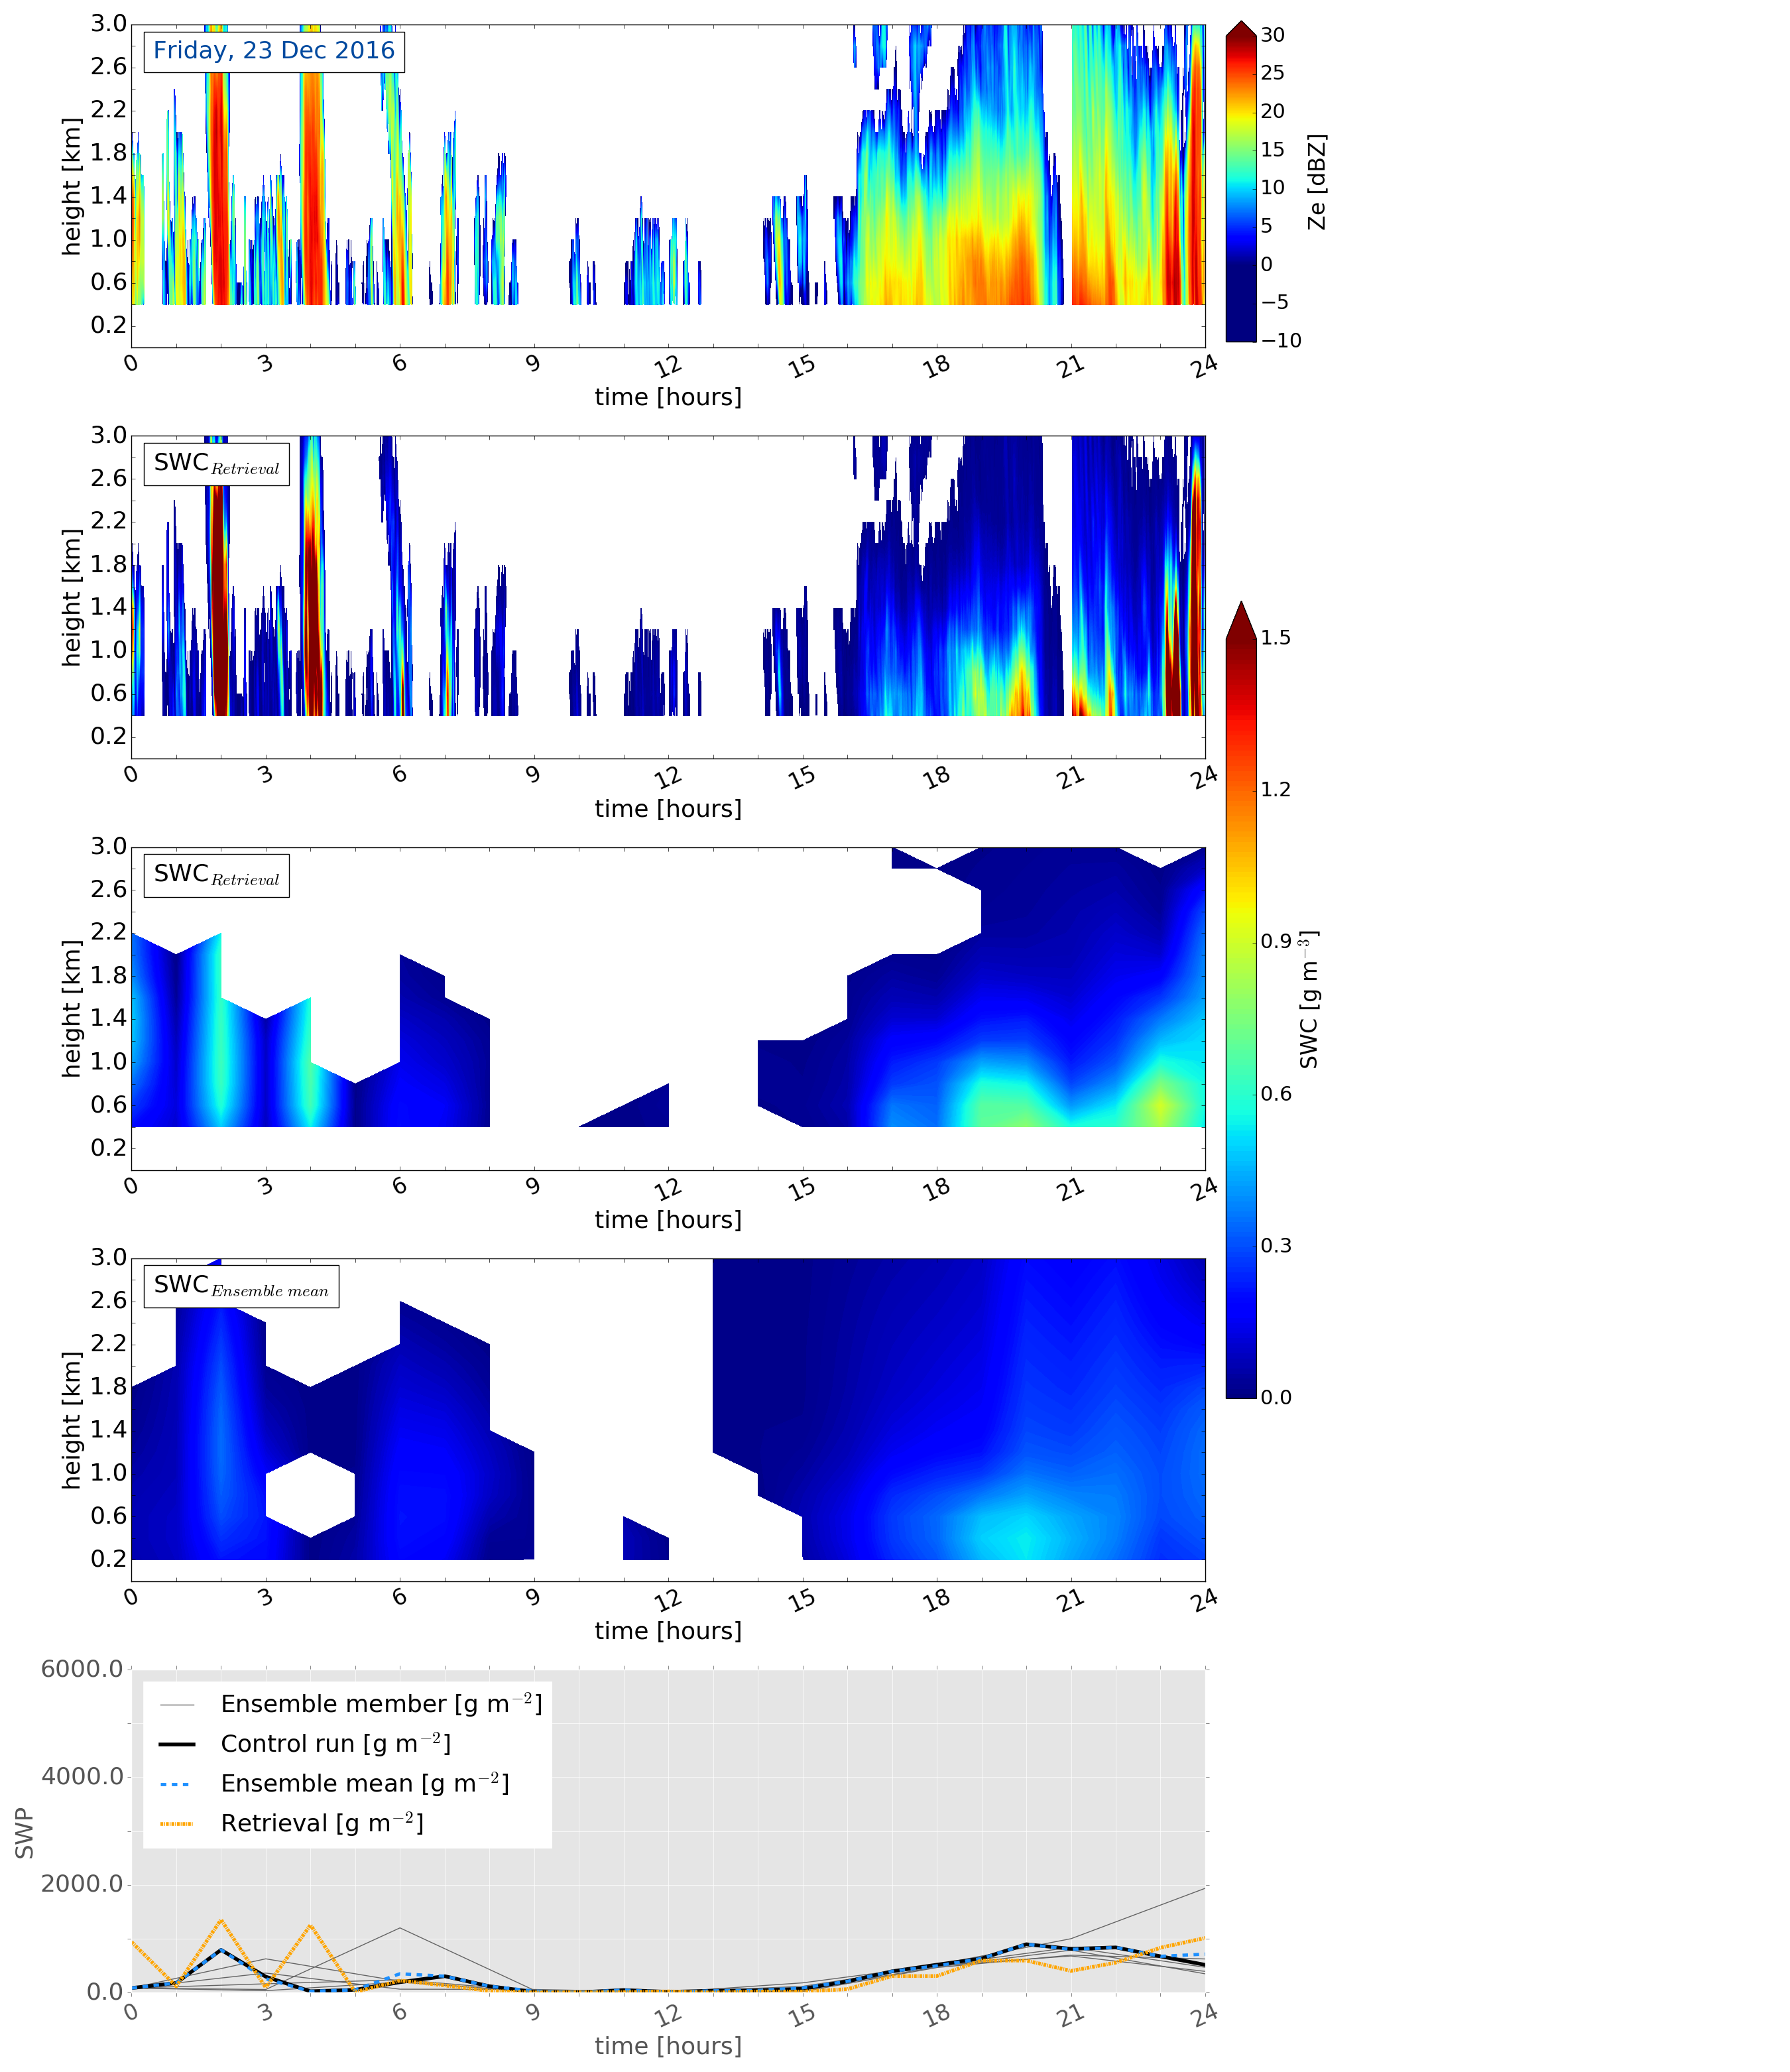
\includegraphics[trim={0.5cm 0.5cm 17.5cm .5cm},clip,width=\textwidth]{./fig_SWC/20161223}
			\caption{Friday, \SI{23}{\dec}}\label{fig:SWC23}
		\end{subfigure}
	\end{figure}
    \begin{figure}\ContinuedFloat
   		\centering
		% 24/12
		\begin{subfigure}[b]{0.8\textwidth}
			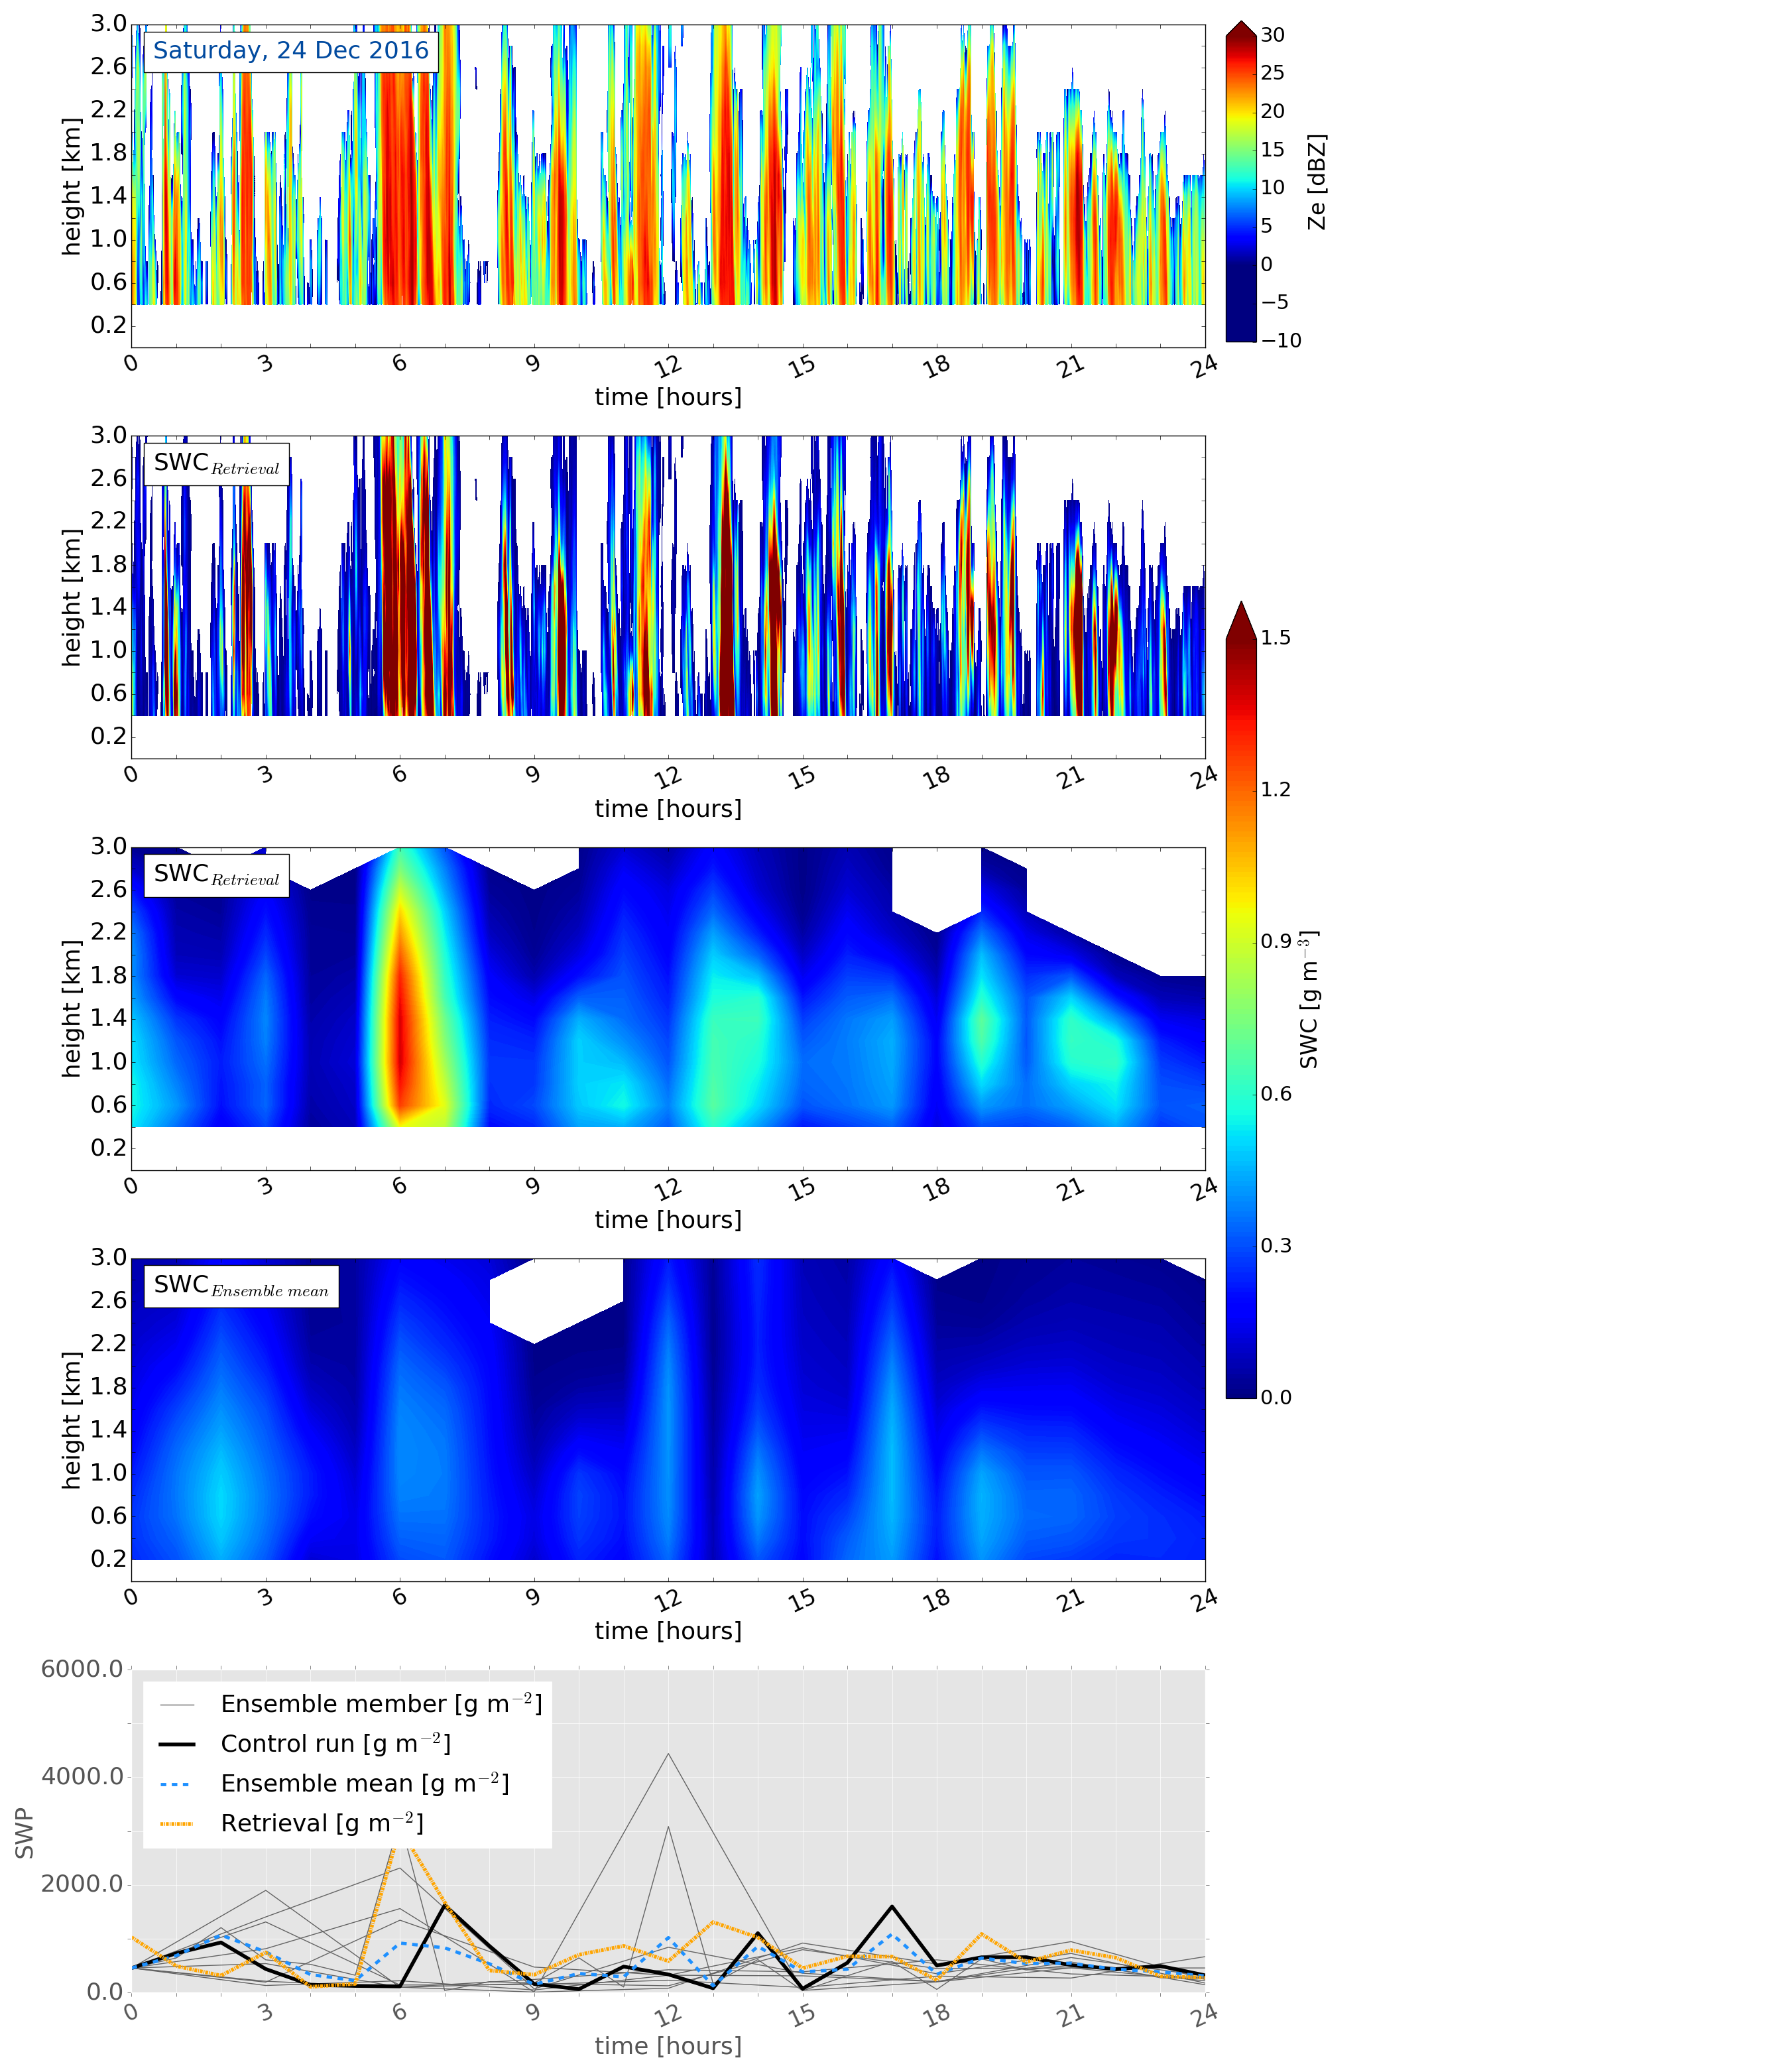
\includegraphics[trim={0.5cm 0.5cm 17.5cm .5cm},clip,width=\textwidth]{./fig_SWC/20161224}
			\caption{Saturday, \SI{24}{\dec}}\label{fig:SWC24}
		\end{subfigure}
	\end{figure}
    \begin{figure}\ContinuedFloat
   		\centering
		% 25/12
		\begin{subfigure}[b]{0.8\textwidth}
			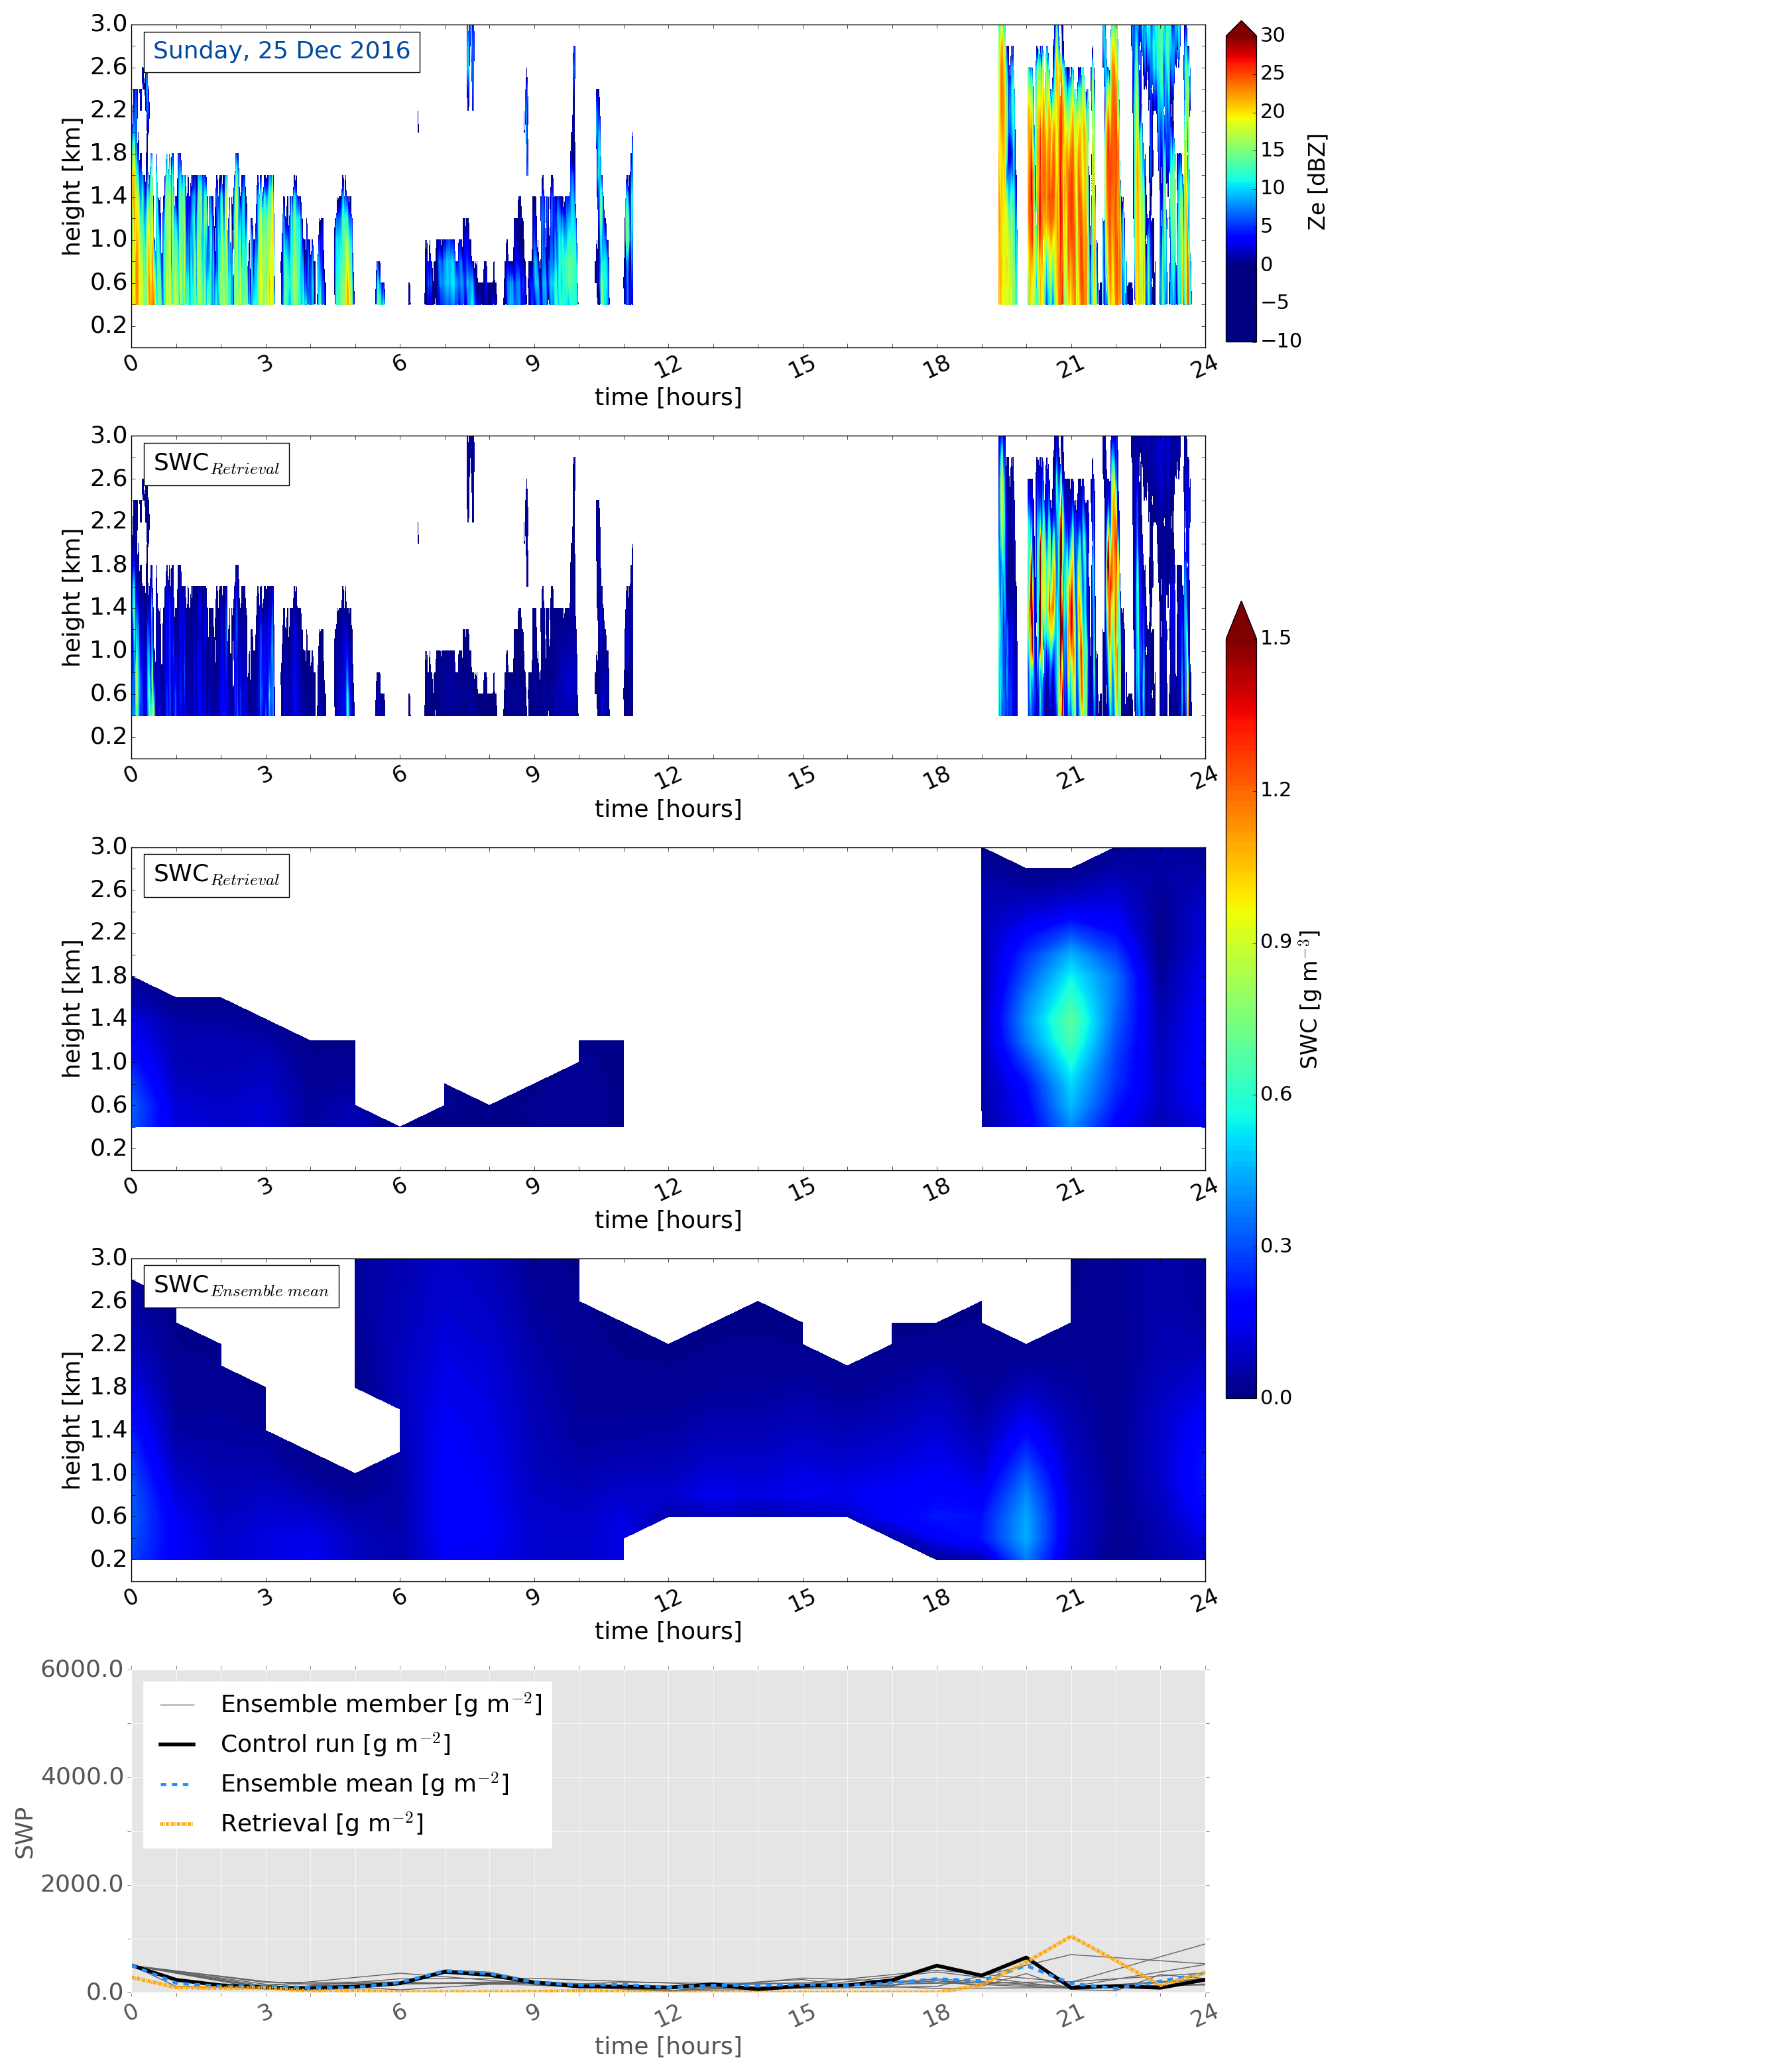
\includegraphics[trim={0.5cm 0.5cm 17.5cm .5cm},clip,width=\textwidth]{./fig_SWC/20161225}
			\caption{Sunday, \SI{25}{\dec}}\label{fig:SWC25}
		\end{subfigure}
	\end{figure}
    \begin{figure}\ContinuedFloat
   		\centering
		% 26/12
		\begin{subfigure}[b]{0.8\textwidth}
			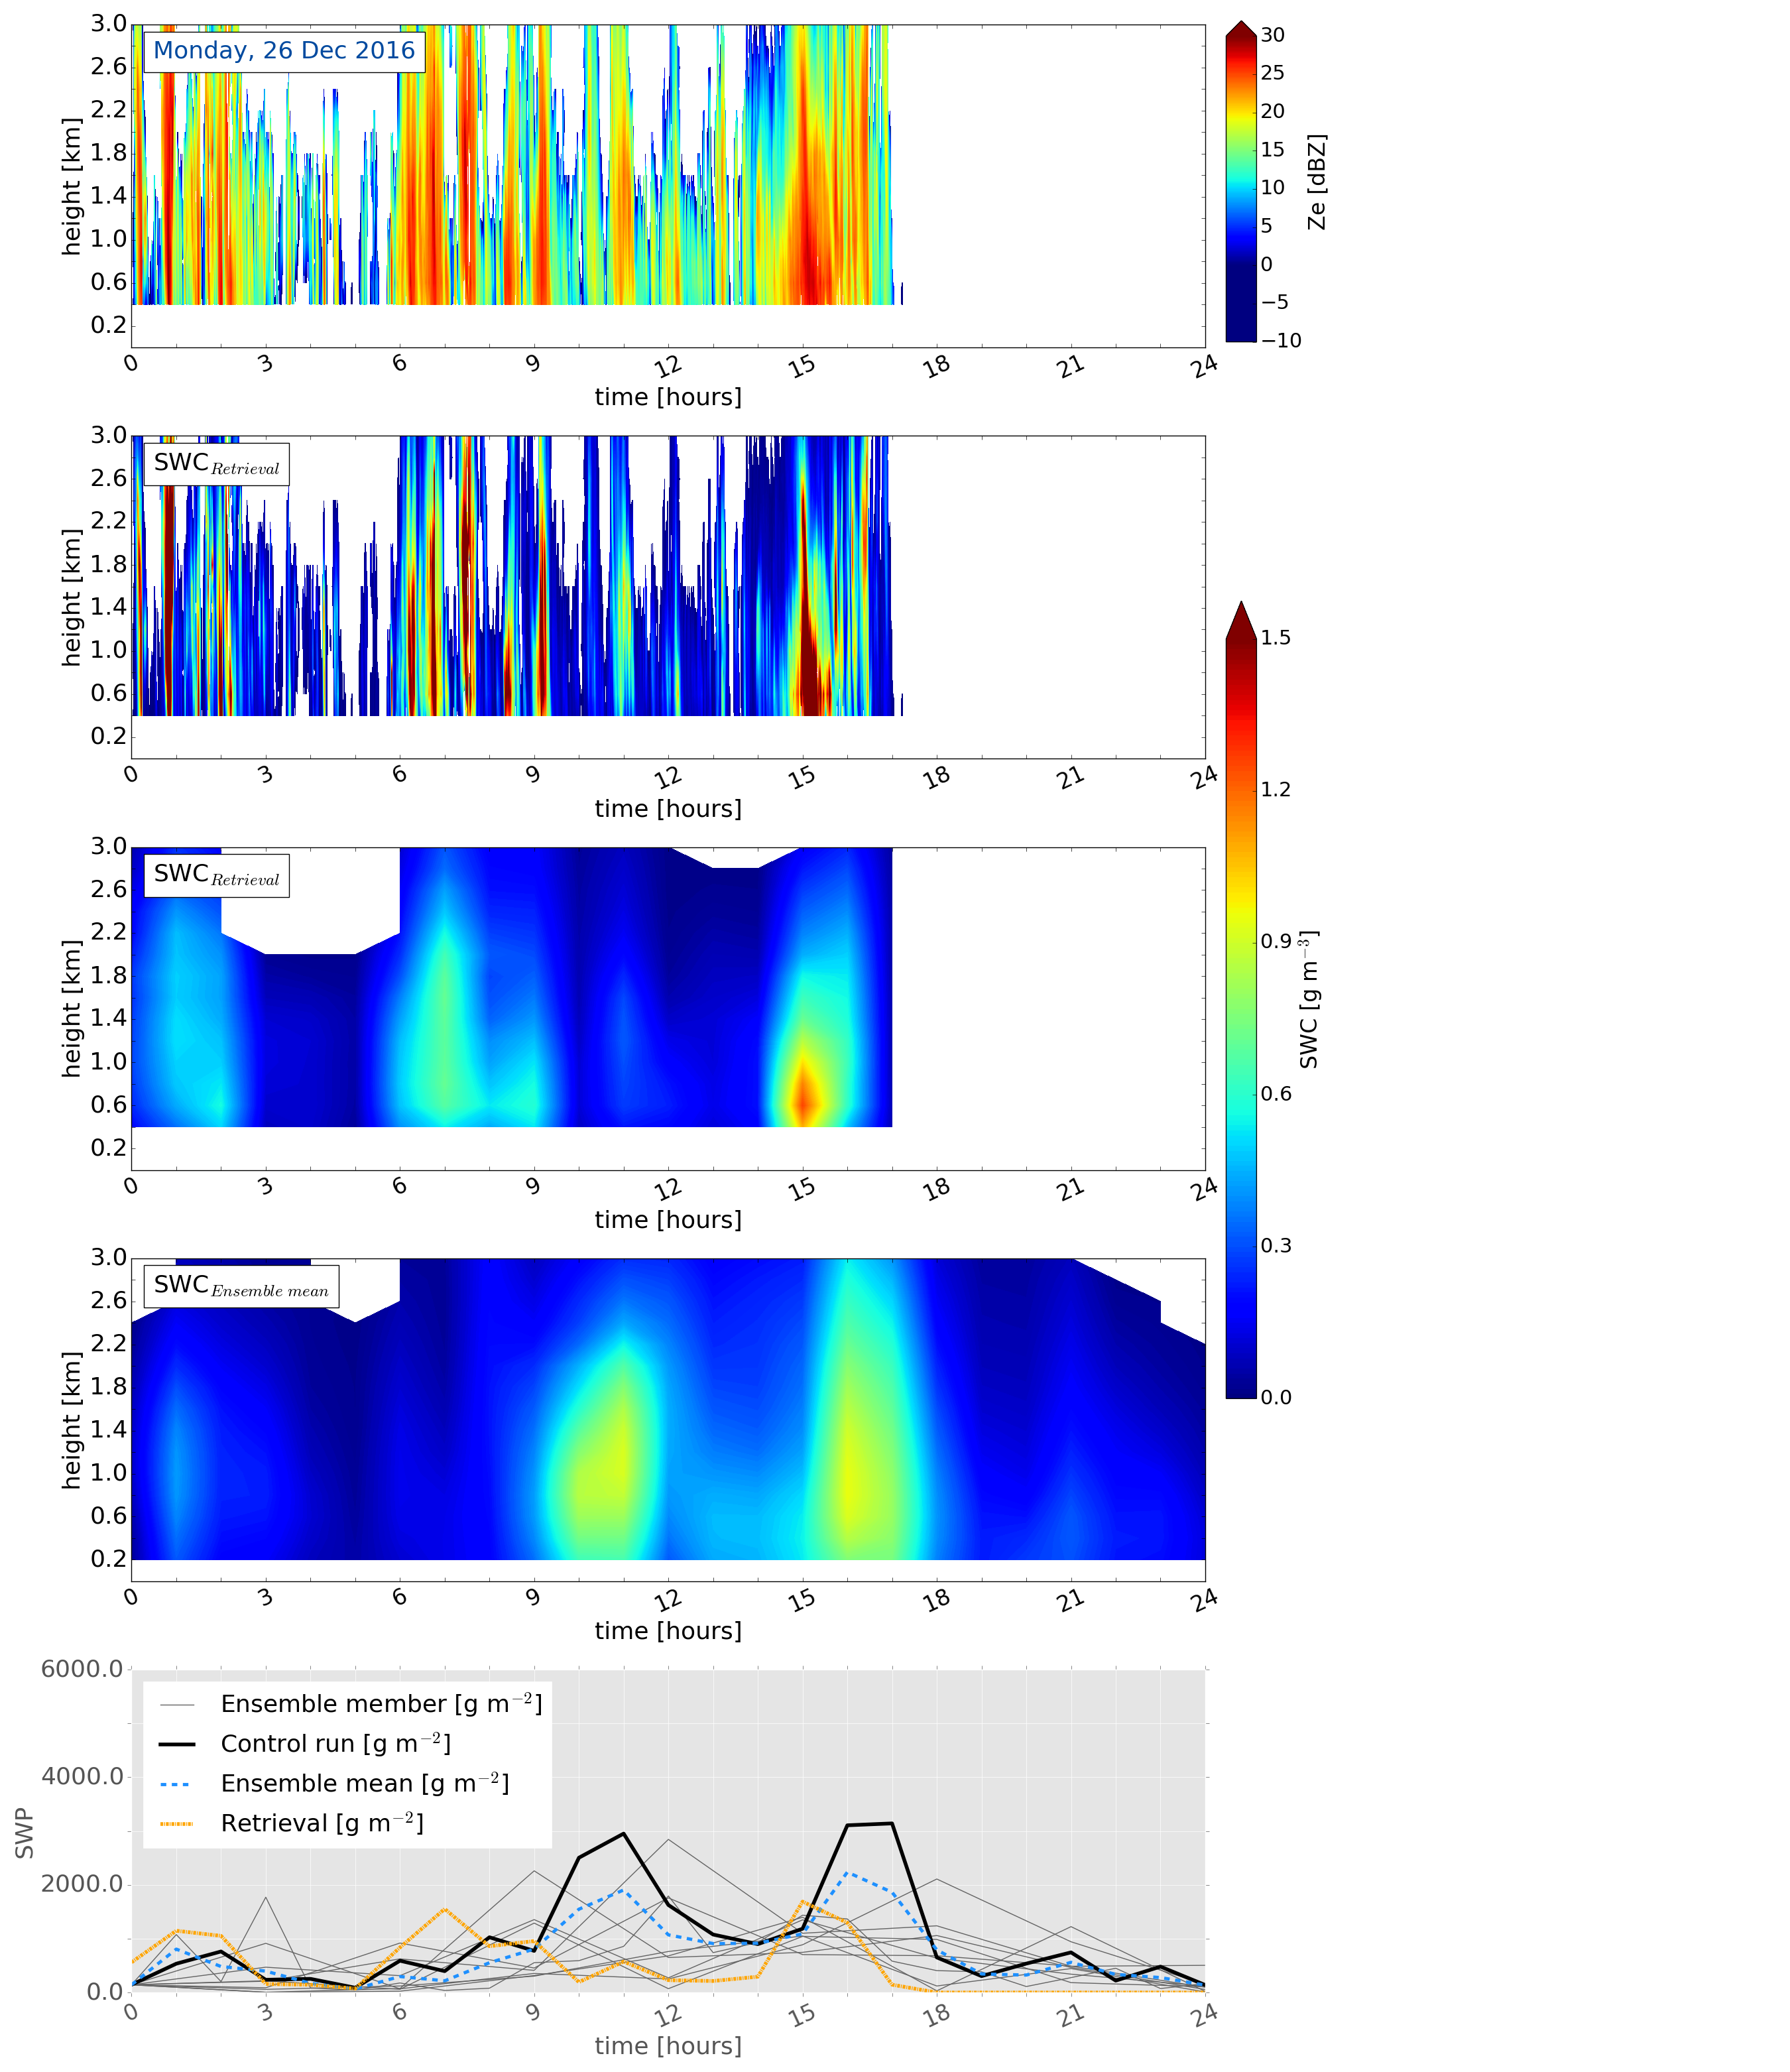
\includegraphics[trim={0.5cm 0.5cm 17.5cm .5cm},clip,width=\textwidth]{./fig_SWC/20161226}
			\caption{Monday, \SI{26}{\dec}}\label{fig:SWC26}
		\end{subfigure}
        \caption{Upper panel: MRR reflectivity in \SI{}{\dB Z}. 2nd panel: SWC optimal estimation retrieval output every second in \SI{}{\gram\per\cubic\metre}. 3rd panel: hourly-averaged SWC optimal estimation retrieval output. 4th panel: \SI{200}{\metre}-averaged SWC deterministic forecast from MEPS. Lowest panel: SWP from MEPS, initialised at \SI{00}{\UTC}. Black line represents the deterministic forecast and the grey lines the nine perturbed members. In blue the SWP from the averaged retrieval output.}\label{fig:SWC}
	\end{figure}
	

%%%%%%%%%%%%%%%%%%%%%%%%%%%%%%%%%%%%%%%%%%%%%%%%%%%%%%%%%%%%%%%%%%%%%%%%%
\section{Vertical Snow Water Content retrieved from optimal estimation and MEPS \SI{48}{\hour} forecast}
The vertical observations from the MRR and the results of the snowfall retrieval for \SIrange{20}{27}{\dec} are presented in the three upper panels of \Cref{fig:SWC20,fig:SWC21,fig:SWC22,fig:SWC23,fig:SWC24,fig:SWC25}. The first panel shows the transformed radar reflectivity in [\SI{}{\decibel Z}], excluding values, were the surface temperature exceeds \SI{2}{\celsius} and reflectivities lower than \SI{-15}{\decibel Z}. After the application of the optimal estimation retrieval, the minutely snow water content is shown in the second panel in \Cref{fig:SWC}. The third panel in \Cref{fig:SWC} shows the hourly averaged SWC from the optimal estimation retrieval. The forecast ensemble mean of all ten ensemble members of MEPS, averaged over \SI{200}{\metre} layers is shown in the forth panel. Although ensemble member two to nine have only data every third hour, the ensemble mean was generated every hour. On hours when there was only the deterministic and the first ensemble member, it can cause that the SWC is slightly higher compared to the three hour values when all ten ensemble member existed. A variation of the SWC of all ten ensemble members is described in \Cref{sec:variation} and the vertical SWC of each ensemble for \SIlist{21;24;25}{\dec} are presented in \Cref{sec:vertEM09:2112,sec:vertEM09:2412,sec:vertEM09:2512}
\\
\\
\Cref{fig:SWC20} shows the SWC for an initialisation on \SI{20}{\dec} at \SI{0}{\UTC}. With a forecast time more than \SI{24}{\hour} prior to the actual precipitation, MEPS does not catch the intensity of the storm. The upper panel in \Cref{fig:SWC20} shows an up-slope event (wind from the east, compare \Cref{fig:site:kartverket}) between \SIlist{9;13}{\UTC}. This turned afterwards into a pulsing event with intense precipitation, resulting in higher reflectivity and therefore higher SWC of more than \SI{1.5}{\SWC}, for durations of about half an hour. The association between up-slope winds and therefore more consistent storm structure, can be seen from the wind barbs in \Cref{fig:sfc_acc21}. Up-slope storms are associated with weaker south-east winds and pulsing with stronger wind from the west. 
When comparing the MEPS forecast initialised on \SI{21}{\dec} at \SI{00}{\UTC}, third and forth panel in \Cref{fig:SWC21}, it shows, that the numerical forecast model captures the up-slope part of the storm, much weaker but around the same time as observed with the MRR. Furthermore captures MEPS some of the pulses occurring after \SI{15}{\UTC} with a peak of \SI{1.24}{\SWC} at \SI{20}{\UTC}, which is in the observations much weaker at this time. An in-depth analysis of \SI{21}{\dec} is given in \Cref{sec:vertEM09:2112}.  %
\\
The \SI{22}{\dec} is dominated by south-west to west wind. As \Cref{fig:SWC21} and \ref{fig:SWC22} show, is this associated with a pulsing of precipitation. High retrieved SWC values are observed by the MRR at \SI{9}{\UTC}. The \SI{24}{\hour} prior initialisation of MEPS indicates some of the pulsing during \SI{22}{\dec}. A forecast started at \SI{0}{\UTC} on \SI{22}{\dec} smears the pulsing more out and also weakens the averaged SWC of the ensemble mean compared to the initialisation on \SI{21}{\dec}, but the pulsing of the event is present in both cases. 
\\
In the evening of \SI{23}{\dec} the wind turns from west to south, again the up-slope wind creates a more consistent storm after around \SI{16}{\UTC} and does not break up the storm structure with a peak of high SWC between \SIrange{20}{22}{\UTC} (\Cref{fig:SWC22} and \ref{fig:SWC23}). Since the wind turns back to west, the maximum value of the hourly averaged SWC is found at \SI{23}{\UTC}. Already on \SI{22}{\dec} one can predict the more consistent up-slope storm in the evening of \SI{23}{\dec}, although weak. An initialisation at \SI{0}{\UTC} on \SI{23}{\dec} intensifies the pulses in the morning and reaches slightly higher values when an up-slope storm is observed.
\\
The \SI{24}{\dec} is dominated by strong west winds and therefore associated with a pulsing event. The SWC obtained by the optimal estimation retrieval reaches its peak at \SI{6}{\UTC} in \Cref{fig:SWC23} and \ref{fig:SWC24}. The MEPS forecast, initiated on \SI{23}{\dec}, shows already the structure of an pulsing event. Comparing the initialisation at \SI{24}{\dec} (forth panel in \Cref{fig:SWC24}), matches the ensemble mean the structure of the observed pulsing of the storms precipitation. Even though the maximum of \SI{1.39}{\SWC} was observed around \SI{6}{\UTC} and MEPS had a SWC maximum value of \SI{0.51}{\SWC} at around \SI{2}{\UTC} is the key, that MEPS already records the structure of the storm more than \SI{24}{\hour} before the event. A detailed description and discussion for \SI{24}{\dec} is given in \Cref{sec:vertEM09:2412}.
\\
In the observations on the \SI{25}{\dec} it shows a gap between \SIrange{11}{19}{\UTC} in the observations in \Cref{fig:SWC24} and \ref{fig:SWC25}. This blank is associated with the fact, that the snowfall retrieval assumes to have the presence of rain, if the surface temperature exceeds \SI{2}{\celsius} and or the reflectivity value is less than \SI{- 15}{\decibel Z}. Until noon show the observations weak snowfall and after the assumed rain a pulsing storm with associated west wind is observed from \SIrange{19}{24}{\UTC}. Neither the MEPS initialisation on \SI{24}{\dec} nor on \SI{25}{\dec} estimates the observed pattern on \SI{25}{\dec}. MEPS predicts a weak peak just after the rain when initialised less than \SI{24}{\hour} in advance. But, it seems that MEPS predicts the liquid water content (LWC) correctly in height and duration between \SIrange{12}{18}{\UTC}. The MRR reflectivity shows high values up to  \SI{1.2}{\kilo\metre} during \SIrange{16}{20}{\UTC}, shown in \Cref{fig:MRR_sfcT}. The sum of cloud water content and rainfall amount from MEPS in \Cref{fig:LWC24} and \ref{fig:LWC25} show high LWC amount during that specific time with maximum values of \SI{0.32}{\SWC} at \SI{17}{\UTC} for an initialisation on \SI{25}{\dec} at \SI{0}{\UTC}. Also, in the vertical figures for the SWC (\Cref{fig:SWC24} and \ref{fig:SWC25}) the liquid layer after noon can be estimated since the values are zero and just above this layer are some lighter blue peaks which indicate a snow water content up to \SI{0.5}{\SWC}.
\\
On \SI{26}{\dec} only retrieved SWC until \SI{17}{\UTC} is valid and comparable, as the reflectivity in the first panel of \Cref{fig:SWC25} and \ref{fig:SWC26} shows. After approximately \SI{17}{\UTC} did the MRR not respond. 
The observations show a pulsing, again related to the west wind over the mountain, close to Haukeliseter. As for \SI{24}{\dec} covers MEPS this pulsing quite well in both, the \SIlist{24;48}{\hour} forecast and even gives an idea how the observations might have been. The maximum SWC value of \SI{1.25}{\SWC} was observed in the hourly averaged retrieved snow water content (third panel \Cref{fig:SWC26}) at \SI{15}{\UTC}, were the ensemble mean showed a daily maximum value of \SI{0.95}{\SWC} at \SI{16}{\UTC}. The purpose of this work is to show, that MEPS forecasts cover the observed snow water content. Even though the ensemble mean might not have reached the maximum value or even covered the same time, a delay of \SIrange{1}{2}{\hour} is a good performance of the regional ensemble model. Comparing the SWC initialised on \SI{25}{\dec} for the \SI{26}{\dec}, it shows more pulsing similar to the observations than an initialisation on \SI{26}{\dec}.
